%%**************************************************************
%% Vorlage fuer Bachelorarbeiten (o.ä.) der DHBW
%%
%% Autor: Tobias Dreher, Yves Fischer
%% Datum: 06.07.2011
%%**************************************************************

\newcommand{\pdftitel}{Title of the document}
\newcommand{\autor}{Max Mustermann}
\newcommand{\arbeit}{Bachelor thesis}

%
% Nahezu alle Einstellungen koennen hier getaetigt werden
%

\documentclass[%
	pdftex,
	oneside,        % Einseitiger Druck.
	12pt,           % Schriftgroesse
	parskip=half,   % Halbe Zeile Abstand zwischen Absätzen.
	headsepline,    % Linie nach Kopfzeile.
	footsepline,    % Linie vor Fusszeile.
	abstracton,     % Abstract Überschriften
	english,        % Translator
]{scrreprt}

%Seitengroesse
\usepackage{fullpage}

%Zeilenumbruch und mehr
\usepackage[activate]{microtype}

% Zeichencodierung
\usepackage[utf8]{inputenc}
\usepackage[T1]{fontenc}

% Zeilenabstand
\usepackage[onehalfspacing]{setspace}

% Index-Erstellung
\usepackage{makeidx}

% Lokalisierung (englische Sprache)
\usepackage[english]{babel}

% Anführungszeichen 
\usepackage[babel,german=quotes]{csquotes}
%\usepackage[style=swiss]{csquotes}


% Spezielle Tabellenform fuer Deckblatt
\usepackage{longtable}
\setlength{\tabcolsep}{10pt} %Abstand zwischen Spalten
\renewcommand{\arraystretch}{1.5} %Zeilenabstand

% Grafiken
\usepackage{graphicx}

% Mathematische Textsaetze
%\usepackage{amsmath}
%\usepackage{amssymb}

% Pakete um Textteile drehen zu können, oder eine Seite Querformat anzeigen kann.
%\usepackage{rotating}
%\usepackage{lscape}

% Farben
\usepackage{color}
\definecolor{LinkColor}{rgb}{0,0,0.2}
\definecolor{ListingBackground}{rgb}{0.92,0.92,0.92}

% PDF Einstellungen
\usepackage[%
	pdftitle={\pdftitel},
	pdfauthor={\autor},
	pdfsubject={\arbeit},
	pdfcreator={pdflatex, LaTeX with KOMA-Script},
	pdfpagemode=UseOutlines, % Beim Oeffnen Inhaltsverzeichnis anzeigen
	pdfdisplaydoctitle=true, % Dokumenttitel statt Dateiname anzeigen.
	pdflang=eng % Sprache des Dokuments.
]{hyperref}

% (Farb-)einstellungen für die Links im PDF
\hypersetup{%
	colorlinks=false, % Aktivieren von farbigen Links im Dokument
	linkcolor=LinkColor, % Farbe festlegen
	citecolor=LinkColor,
	filecolor=LinkColor,
	menucolor=LinkColor,
	urlcolor=LinkColor,
	bookmarksnumbered=true % Überschriftsnummerierung im PDF Inhalt anzeigen.
}

% Verschiedene Schriftarten
%\usepackage{goudysans}
%\usepackage{lmodern}
%\usepackage{libertine}
\usepackage{palatino} 

% Hurenkinder und Schusterjungen verhindern
% http://projekte.dante.de/DanteFAQ/Silbentrennung
\clubpenalty=10000
\widowpenalty=10000
\displaywidowpenalty=10000

% Quellcode
\usepackage{listings}
\lstloadlanguages{Java}
\lstset{%
	language=PHP,            % Sprache des Quellcodes
	%numbers=left,           % Zeilennummern links
	stepnumber=1,            % Jede Zeile nummerieren.
	numbersep=5pt,           % 5pt Abstand zum Quellcode
	numberstyle=\tiny,       % Zeichengrösse 'tiny' für die Nummern.
	breaklines=true,         % Zeilen umbrechen wenn notwendig.
	breakautoindent=true,    % Nach dem Zeilenumbruch Zeile einrücken.
	postbreak=\space,        % Bei Leerzeichen umbrechen.
	tabsize=2,               % Tabulatorgrösse 2
	basicstyle=\ttfamily\footnotesize, % Nichtproportionale Schrift, klein für den Quellcode
	showspaces=false,        % Leerzeichen nicht anzeigen.
	showstringspaces=false,  % Leerzeichen auch in Strings ('') nicht anzeigen.
	extendedchars=true,      % Alle Zeichen vom Latin1 Zeichensatz anzeigen.
	captionpos=b,            % sets the caption-position to bottom
	backgroundcolor=\color{ListingBackground} % Hintergrundfarbe des Quellcodes setzen.
}

% Glossar
\usepackage[
	nonumberlist, %keine Seitenzahlen anzeigen
	acronym,      %ein Abkürzungsverzeichnis erstellen
	%section,     %im Inhaltsverzeichnis auf section-Ebene erscheinen
	toc,          %Einträge im Inhaltsverzeichnis
]{glossaries}

% Fussnoten
\usepackage[perpage, hang, multiple, stable]{footmisc}

% Titel, Autor und Datum
\title{\titel}
\author{\autor}
\date{\datum}


% Ab jetzt können auch Umlaute verwendet werden
\newcommand{\titel}{Usually the title of a Bachelor thesis has a length of two lines}
\newcommand{\matrikelnr}{1234567}
\newcommand{\kurs}{ABC2008DE}
\newcommand{\datumAbgabe}{August 2011}
\newcommand{\firma}{Firma GmbH}
\newcommand{\firmenort}{Firmenort}
\newcommand{\abgabeort}{Abgabeort}
\newcommand{\abschluss}{Bachelor of Arts}
\newcommand{\studiengang}{Vorderasiatische Archäologie}
\newcommand{\dhbw}{Stuttgart Campus Horb}
\newcommand{\betreuer}{Dipl.-Ing. (FH) Peter Pan}
\newcommand{\gutachter}{Dr. Silvana Koch-Mehrin}
\newcommand{\zeitraum}{12 Weeks}

\makeglossaries
%
% vorher in Konsole folgendes aufrufen: 
%	makeglossaries makeglossaries dokumentation.acn && makeglossaries dokumentation.glo
%

%
% Abkürzungen --> referenz, name, beschreibung
% Aufruf mit \gls{...} oder Kurzform mit \acrshort{...}
%

\newacronym{DHBW}{DHBW}{Duale Hochschule Baden Württemberg}
\newacronym{I2CBus}{I\textsuperscript{2}C-Bus}{Inter-Integrated-Circuit-Bus}

%
% Glossareintraege --> referenz, name, beschreibung
% Aufruf mit \gls{...}
%
\newglossaryentry{Glossareintrag}{name={Glossareintrag},plural={Glossareinträge},description={Ein Glossar beschreibt verschiedenste Dinge in kurzen Worten}}


\begin{document}

	% Deckblatt
	\begin{spacing}{1}
		\begin{titlepage}
	\begin{longtable}{p{.55\textwidth} p{.85\textwidth}}
	  {\includegraphics[height=2.6cm]{images/logo.png}} & 
	  {
\includegraphics[height=2.6cm]{images/dhbw.png}}
	\end{longtable}
	\enlargethispage{20mm}
	\begin{center}
	  \vspace*{12mm}	{\LARGE\bf \titel }\\
	  \vspace*{12mm}	{\large\bf \arbeit}\\
	  \vspace*{12mm}	for the\\
	  \vspace*{3mm} 	{\bf \abschluss}\\
	  \vspace*{12mm}	at Course of Studies \studiengang\\
	  \vspace*{3mm} 	at the Cooperative State University \dhbw\\
	  \vspace*{12mm}	by\\
	  \vspace*{3mm} 	{\large\bf \autor}\\
	  \vspace*{12mm}	\datumAbgabe\\
	\end{center}
	\vfill
	\begin{spacing}{1.2}
	\begin{tabbing}
		mmmmmmmmmmmmmmmmmmmmmmmmmm     \= \kill
		\textbf{Time of Project}  \>  \zeitraum\\
		\textbf{Student ID, Course}  \>  \matrikelnr, \kurs\\
		\textbf{Company}      \>  \firma, \firmenort\\
		\textbf{Supervisor in the Company}              \>  \betreuer\\
		\textbf{Reviewer}             \>  \gutachter
	\end{tabbing}
	\end{spacing}
\end{titlepage}

	\end{spacing}
	\newpage
	
	\renewcommand{\thepage}{\Roman{page}}
	\setcounter{page}{1}
	
	% Erklärung
	\thispagestyle{empty}

\section*{Author's declaration}
% Seite 8
% http://studium.ba-bw.de/fileadmin/media/allgemein/bestimmungen/btechnik/richtlinien/Richtlinien_Praxismodule_Studien_und_Bachelorarbeiten_2011.pdf
\vspace*{2em}
Unless otherwise indicated in the text or references, or acknowledged above, this thesis is entirely the product of my own scholarly work. This thesis has not been submitted either in whole or part, for a degree at this or any other university or institution. This is to certify that the printed version is equivalent to the submitted electronic one.
\vspace{3em}

\abgabeort, \datumAbgabe
\vspace{4em}

\rule{6cm}{0.4pt}\\
\autor



	\newpage

	% Abstract
	\thispagestyle{empty}

\renewcommand{\abstractname}{Zusammenfassung}
\begin{abstract}
Ein Abstract ist eine prägnante Inhaltsangabe, ein Abriss ohne
Interpretation und Wertung einer wissenschaftlichen Arbeit. In DIN
1426 wird das (oder auch der) Abstract als Kurzreferat zur
Inhaltsangabe beschrieben.

\begin{description}
\item[Objektivität] soll sich jeder persönlichen Wertung enthalten
\item[Kürze] soll so kurz wie möglich sein
\item[Genauigkeit] soll genau die Inhalte und die Meinung der Originalarbeit wiedergeben
\end{description}

Üblicherweise müssen wissenschaftliche Artikel einen Abstract
enthalten, typischerweise von 100-150 Wörtern, ohne Bilder und
Literaturzitate und in einem Absatz.

Quelle \url{http://de.wikipedia.org/wiki/Abstract} Abgerufen 07.07.2011
\end{abstract}


\renewcommand{\abstractname}{Summary}
\begin{abstract}
An abstract is a brief summary of a research article, thesis, review,
conference proceeding or any in-depth analysis of a particular subject
or discipline, and is often used to help the reader quickly ascertain
the paper's purpose. When used, an abstract always appears at the
beginning of a manuscript, acting as the point-of-entry for any given
scientific paper or patent application. Abstracting and indexing
services for various academic disciplines are aimed at compiling a
body of literature for that particular subject.

The terms précis or synopsis are used in some publications to refer to
the same thing that other publications might call an "abstract". In
management reports, an executive summary usually contains more
information (and often more sensitive information) than the abstract
does.

Quelle: \url{http://en.wikipedia.org/wiki/Abstract_(summary)}

\end{abstract}

	\newpage

	\pagestyle{plain}

	% Inhaltsverzeichnis
	\begin{spacing}{1.1}
		\setcounter{tocdepth}{3}
		\tableofcontents
	\end{spacing}
	\newpage

	\renewcommand{\thepage}{\arabic{page}}
	\setcounter{page}{1}

	% Inhalt
	\chapter{Das erste Kapitel}
\section{Using Abbreviations, Glossary and References}
\subsection{Abbreviations}
\subsubsection{Per Glossar}
Abbreviations short: \acrshort{DHBW}, \acrshort{I2CBus} 

and written out: \gls{DHBW}, \gls{I2CBus}

\subsubsection{Per acronym package}
Erste Erwähnung eines Akronyms wird ausgeschrieben mit Akürzung in Klammern angezeigt: \ac{AGPL}. Jede weitere wird nur in Kurzform verlinkt. Zweite Erwähnung: mehr zu \ac{AGPL} in \cite{fsf:2007}

\subsection{Citations etc}
References to Glossary:

 Singular: \gls{Glossareintrag}, Plural: \glspl{Glossareintrag}

Meine erste Fußnote\footnote{Ich bin eine Fußnote}

\subsubsection{BibTeX / Biber via blibliographie.bib}
Nur erwähnte Literaturverweise werden auch im Literaturverzeichnis gedruckt:
Indirektes Zitat (vgl. \cite{baumgartner:2002}) oder auch ein ``direktes Zitat'', \cite{dreyfus:1980}.

\textquote[{\cite[p. 35]{baumgartner:2002}}]{Direct citation which might span over several lines and thus should not be placed inline.}

%-----------------------------------------------------
% % possible alignments for wrapped figure:
% 
%    r, R - right side of the text.
%    l, L - left side of the text.
%    i, I - inside edge–near the binding (if [twoside] document).
%    o, O - outside edge–far from the binding.

\begin{wrapfigure}{R}{.4\textwidth}	% right aligned: r, allow to float (capital `R'/'L')
\includegraphics[height=.4\textwidth]{logo.png}
%\vspace{-15pt}	% push 15pt upwards
\caption{Das Logo der Musterfirma\footnotemark} % reference in footnote
\label{fig:logo-muster}
\end{wrapfigure}
\footnotetext{aus \cite{mustermann:2012}} % footnote text for above figure
%-----------------------------------------------------

\subsubsection{Reference via literatur.tex}
This doesn't work when biblatex is used:

\cite{bib:ix042010}, \cite{bib:metasploitBuch}
\paragraph{}
\textquote[{\cite[p. 35]{bib:metasploitBuch}}]{direct citation}.

\section{Figures}
Figure \ref{fig:logo-muster} shows a wrapped image.

Abbildung \ref{fig:ksmswing-diagramm} zeigt, dass ein kleines Bild zentral dargestellt werden kann...

\begin{figure}[ht!]
\centering
\includegraphics{images/logo.png}
%\includegraphics[width=\textwidth]{images/logo.png}
\caption{KSM/Swing Applikation \cite{mustermann:2012}}
\label{fig:ksmswing-diagramm}
\end{figure}


\section{lorem ipsum}
Looking for the one superhero comic you just have to read. Following the antics and adventures of May Mayday Parker, this Spider-book has everything you could want in a comic--action, laughs, mystery and someone in a Spidey suit. Collects Alias \#1-28, What If. Jessica Jones had Joined the Avengers. In her inaugural arc, Jessicas life immediately becomes expendable when she uncovers the potentially explosive secret of one heros true identity.

Once upon a time, Jessica Jones was a costumed super-hero, just not a very good one. First, a story where Wolverine and Hulk come together, and then Captain America and Cable meet up. In a city of Marvels, Jessica Jones never found her niche. The classic adventures of Spider-Man from the early days up until the 90s. Looking for the one superhero comic you just have to read.

	%!TEX root = ../dokumentation.tex

\chapter{Listings and Code}

eingebunden aus c-datei:
\lstinputlisting[language=C,basicstyle=\ttfamily\scriptsize,
caption={simple blinky for STM32F4}]{files/blinky.c}\label{blinky_source}

%title wird unter dem Bsp. abgedruckt
%caption wird im Verzeichnis abgedruckt
%label wird zum referenzieren benutzt, muss einzigartig sein.
Written diretly in \LaTeX \ file:
\begin{lstlisting}[caption=Code-Beispiel, label=Bsp.1]
public class HelloWorld {
	public static void main (String[] args) {
		// Ausgabe Hello World!
		System.out.println("Hello World!");
	}
}
\end{lstlisting}

%language ändert die Sprache. (Wenn nur eine Sprache verwendet wird, kann diese Sprache in einstellungen.tex geändert werden. Standardmäßig Java.)
\begin{lstlisting}[caption=Python-Code, label=Python-Code, title=Titel des Python-Codes,language=Python]
def quicksort(liste):
	if len(liste) <= 1:
		return liste
	pivotelement = liste.pop()
	links = [element for element in liste if element < pivotelement]
	rechts = [element for element in liste if element >= pivotelement]
	return quicksort(links) + [pivotelement] + quicksort(rechts)
# Quelle: http://de.wikipedia.org/wiki/Python_(Programmiersprache)
\end{lstlisting}

\section{Verweis auf Code}
Verweis auf den Code \autoref{Bsp.1}.\\
und der Python-Code \autoref{Python-Code}.

\section{lorem ipsum}
Looking for the one superhero comic you just have to read. Following the antics and adventures of May Mayday Parker, this Spider-book has everything you could want in a comic--action, laughs, mystery and someone in a Spidey suit. Collects Alias \#1-28, What If. Jessica Jones had Joined the Avengers. In her inaugural arc, Jessicas life immediately becomes expendable when she uncovers the potentially explosive secret of one heros true identity.

Once upon a time, Jessica Jones was a costumed super-hero, just not a very good one. First, a story where Wolverine and Hulk come together, and then Captain America and Cable meet up. In a city of Marvels, Jessica Jones never found her niche. The classic adventures of Spider-Man from the early days up until the 90s. Looking for the one superhero comic you just have to read.

Meet all of Spideys deadly enemies, from the Green Goblin and Doctor Octopus to Venom and Carnage, plus see Peter Parker fall in love, face tragedy and triumph, and learn that with great power comes great responsibility. In a city of Marvels, Jessica Jones never found her niche. Bitten by a radioactive spider, high school student Peter Parker gained the speed, strength and powers of a spider. Looking for the one superhero comic you just have to read. What do you get when you ask the question, What if Spider-Man had a daughter.

The classic adventures of Spider-Man from the early days up until the 90s. Amazing Spider-Man is the cornerstone of the Marvel Universe. But will each partner’s combined strength be enough. Adopting the name Spider-Man, Peter hoped to start a career using his new abilities. Youve found it.


	% Anhang
	\clearpage
	\pagenumbering{roman}

	% Abbildungsverzeichnis
	\cleardoublepage
	\phantomsection \label{listoffig}
	\addcontentsline{toc}{chapter}{List of figures}
	\listoffigures

	%Tabellenverzeichnis
	\cleardoublepage
	\phantomsection \label{listoftab}
	\addcontentsline{toc}{chapter}{List of tables}
	\listoftables

	% Quellcodeverzeichnis
	\cleardoublepage
	\phantomsection \label{listoflist}
	\addcontentsline{toc}{chapter}{Listings}
	\lstlistoflistings

	% Literaturverzeichnis
	\cleardoublepage
	\phantomsection \label{listoflit}
	\addcontentsline{toc}{chapter}{Bibliography}
	\begin{thebibliography}{---}

\bibitem[HAM10]{bib:ix042010}
  \textsc{Michael Hamm}: 
  \textbf{Der Erbe wächst - Freier Schwachstellen-Scanner OpenVAS 3.0}.
  iX Magazin, Ausgabe 4/2010, S. 81 ff., Heise Zeitschriften Verlag

\bibitem[NEU11]{bib:metasploitBuch}
  \textsc{Frank Neugebauer}: 
  \textbf{Penetration Testing mit Metasploit}.
  1. Auflage, 2011, dpunkt.verlag GmbH

\end{thebibliography}



	% Abkürzungsverzeichnis
	% vorher in Konsole folgendes aufrufen: 
	%	makeglossaries makeglossaries dokumentation.acn && makeglossaries dokumentation.glo
	\printglossary[type=\acronymtype]

	% Glossar
	\printglossary[style=altlist,title=Glossary]
\end{document}
